\chapter{Games}

In this course, we are interested in two-player games with 
perfect knowledge (both players have the same information on the state of the game).


\section{Minimax algorithm}
\marginnote{Minimax algorithm}
The minimax (min-max) algorithm allows to determine the optimal strategy for a player by
building and propagating utility scores in a tree where each node represents a state of the game.
It considers the player as the entity that maximizes (\textsc{Max}) its utility and
the opponent as the entity that (optimally) minimizes (\textsc{Min}) the utility of the player.


\begin{figure}[h]
    \centering
    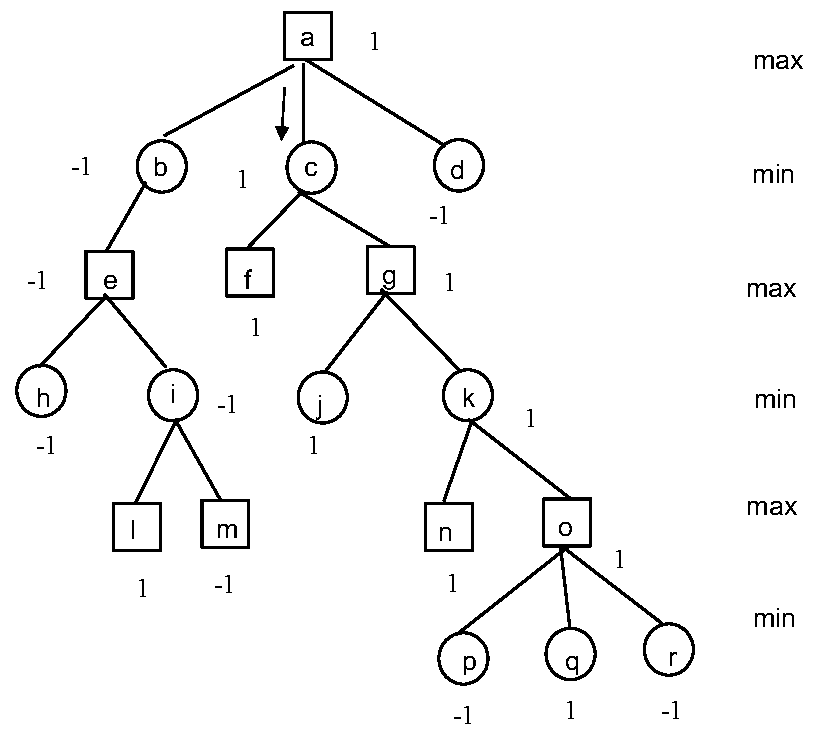
\includegraphics[width=0.5\textwidth]{img/_minmax.pdf}
    \caption{Example of game tree with propagated scores}
\end{figure}

In a game tree, each level represents the actions a that single player can do.
In minimax, the levels where the player plays are the \textsc{Max} levels, 
while the levels of the opponent are the \textsc{Min} levels.

Given a node $n$ of a game tree,
an iteration of the minimax algorithm can be described as follows:
\begin{descriptionlist}
    \item[Expansion] 
        Expansion of the sub-tree having $n$ as root by considering the possible moves starting from the state of $n$.
        
        The expansion in height stops when a final state is reached or when some predetermined conditions are met 
        (note that different branches may be expanded with different heights).

        The expansion in width stops when all the possible moves have been considered or when some predetermined conditions are met.

    \item[Evaluation]
        Each leaf is labeled with a score.
        For terminal states, a possible score assignment is:
        \[ \texttt{utility}(\texttt{state}) = \begin{cases}
            +1 & \text{Win} \\
            -1 & \text{Loss} \\
            0 & \text{Draw}
        \end{cases} \]
        For non-terminal states, heuristics are required.

    \item[Propagation]
        Starting from the parents of the leaves, the scores are propagated upwards 
        by labeling the parents based on the children's score.

        Given an unlabeled node $m$, if $m$ is at a \textsc{Max} level, its label is the maximum of its children's score.
        Otherwise (\textsc{Min} level), the label is the minimum of its children's score.
\end{descriptionlist}


\begin{center}
    \def\arraystretch{1.2}
    \begin{tabular}{c | m{10cm}}
        \hline
        \textbf{Completeness} & Yes, if the game tree is finite \\
        \hline
        \textbf{Optimality} & Yes, assuming an optimal opponent (otherwise, it may need more moves) \\
        \hline
        \textbf{Time complexity}
            & $O(b^m)$, with breadth $m$ and branching factor $b$ \\
        \hline
        \textbf{Space complexity}
            & $O(b \cdot m)$, with breadth $m$ and branching factor $b$ \\
        \hline
    \end{tabular}
\end{center}

\begin{algorithm}
\caption{Minimax algorithm}
\begin{lstlisting}[mathescape=true]
    def minimax(node, max_depth, who_is_next):
        if node.isLeaf() or max_depth == 0: 
            eval = evaluate(node)
        elif who_is_next == ME:
            eval = -$\infty$
            for c in node.children:
                eval = max(eval, minimax(c, max_depth-1, OPPONENT))
        elif who_is_next == OPPONENT:
            eval = +$\infty$
            for c in node.children:
                eval = min(eval, minimax(c, max_depth-1, ME))
        return eval
\end{lstlisting}
\end{algorithm}


\section{Alpha-beta cuts}
\marginnote{Alpha-beta cuts}
Alpha-beta cuts (pruning) allows to prune subtrees whose state will never be selected (when playing optimally).
$\alpha$ represents the best choice found for \textsc{Max}.
$\beta$ represents the best choice found for \textsc{Min}.

The best case for alpha-beta cuts is when the best nodes are evaluated first.
In this scenario, the theoretical number of nodes to explore is decreased to $O(b^{d/2})$.
In practice, the reduction is of order $O(\sqrt{b^d})$.
In the average case of a random distribution, the reduction is of order $O(b^{3d/4})$.

\begin{algorithm}
\caption{Minimax with alpha-beta cuts}
\begin{lstlisting}[mathescape=true]
    def alphabeta(node, max_depth, who_is_next, $\alpha$=-$\infty$, $\beta$=+$\infty$):
        if node.isLeaf() or max_depth == 0: 
            eval = evaluate(node)
        elif who_is_next == ME:
            eval = -$\infty$
            for c in node.children:
                eval = max(eval, alphabeta(c, max_depth-1, OPPONENT, $\alpha$, $\beta$))
                $\alpha$ = max(eval, $\alpha$)
                if eval >= $\beta$: break # cutoff
        elif who_is_next == OPPONENT:
            eval = +$\infty$
            for c in node.children:
                eval = min(eval, alphabeta(c, max_depth-1, ME, $\alpha$, $\beta$))
                $\beta$ = min(eval, $\beta$)
                if eval <= $\alpha$: break # cutoff
        return eval
\end{lstlisting}
\end{algorithm}

\begin{figure}[h]
    \begin{subfigure}{.3\textwidth}
        \centering
        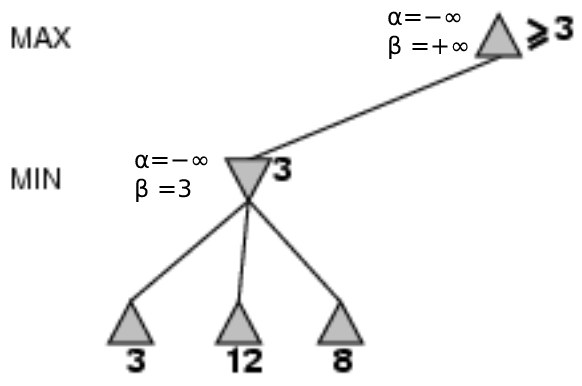
\includegraphics[width=\linewidth]{img/alphabeta_algo_example1.png}
    \end{subfigure}
    \begin{subfigure}{.3\textwidth}
        \centering
        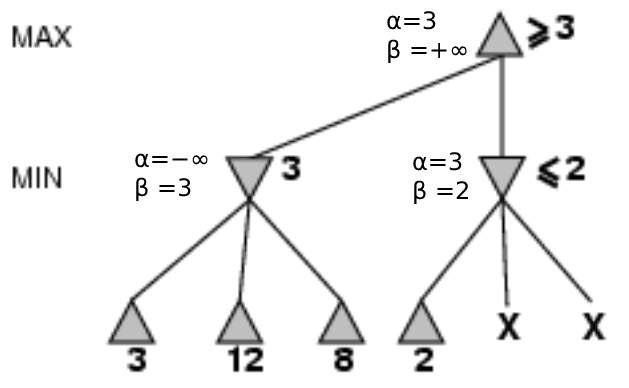
\includegraphics[width=\linewidth]{img/alphabeta_algo_example2.png}
    \end{subfigure}
    \begin{subfigure}{.4\textwidth}
        \centering
        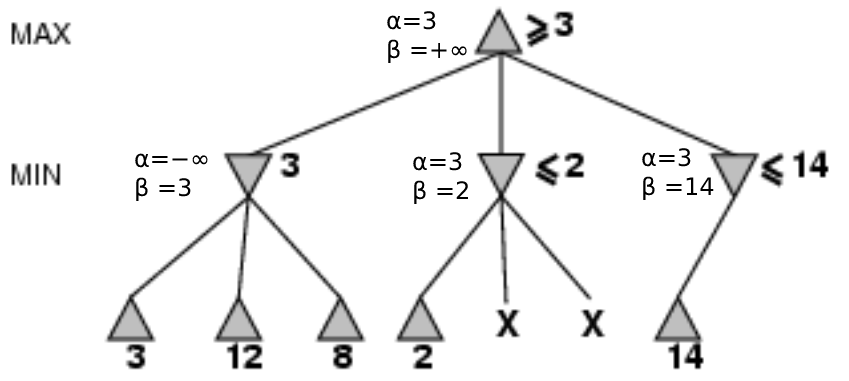
\includegraphics[width=\linewidth]{img/alphabeta_algo_example3.png}
    \end{subfigure}
    \begin{subfigure}{.4\textwidth}
        \centering
        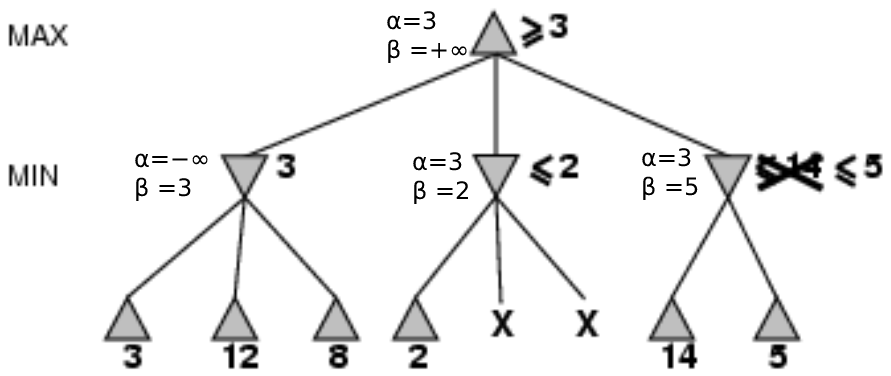
\includegraphics[width=\linewidth]{img/alphabeta_algo_example4.png}
    \end{subfigure}
    \begin{subfigure}{.4\textwidth}
        \centering
        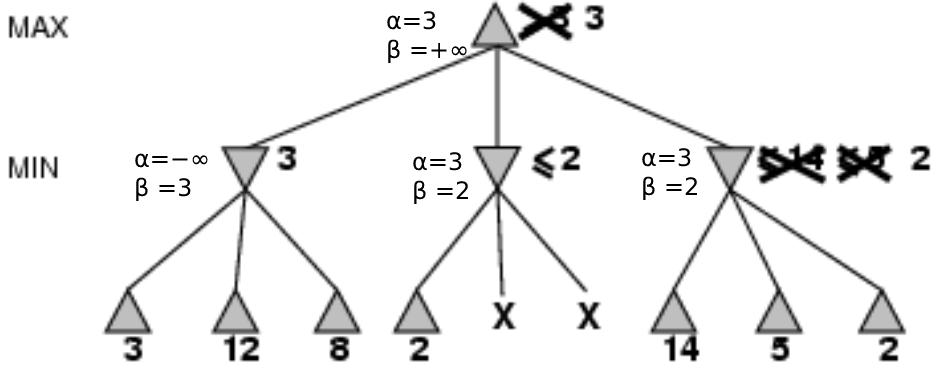
\includegraphics[width=\linewidth]{img/alphabeta_algo_example5.png}
    \end{subfigure}
    \caption{Algorithmic (left) and intuitive (right) application of alpha-beta cuts}
\end{figure}